\documentclass[11pt,letterpaper]{article}
\title{Plant Generator}
\date{\today}
\usepackage[margin=1in]{geometry}
\usepackage{float}
\usepackage{tikz}
\usetikzlibrary{arrows.meta}
\tikzset{
>={Latex[width=2mm,length=2mm]},
	box1/.style={
		rectangle,
		sharp corners,
		fill=black!0,
		draw=black, very thick,
		text width=10em,
		minimum height=3em,
		text centered},
	box2/.style={
		rectangle,
		sharp corners,
		fill=black!0,
		draw=black, very thick,
		text width=3em,
		minimum height=3em,
		text centered}
}

\makeatletter
\begin{document}
\begin{center}
	\begin{huge} \@title \end{huge} \\
	\vspace{1em}
	\begin{LARGE} Documentation \end{LARGE} \\
	\vspace{1em}
	\@date
\end{center}
\tableofcontents
\pagebreak

\section{Introduction}

The project is split in two parts. The editor component handles all user input and provides realtime feedback. The generator component defines and generates the plant structure, which is used to create a plant mesh. It is intended that the generator is removable from the editor so that it can be used as a library instead. Plants are generated preferably from environmental input if the generator is used as a library.

\vspace{2em}
\begin{figure}[H]
\centering
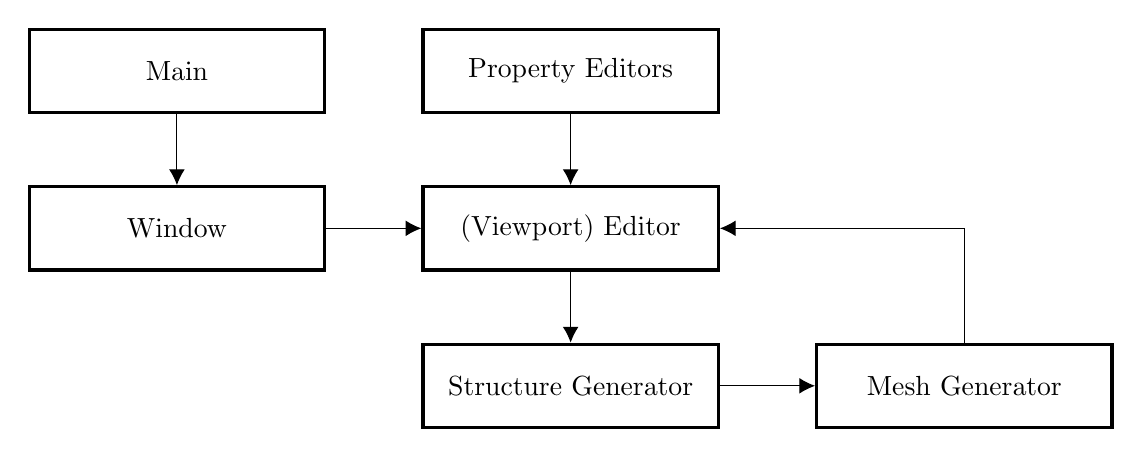
\begin{tikzpicture}
[node distance=2cm]
\node[box1] (main) {Main};
\node[box1, below of=main, xshift=0cm] (window) {Window};
\node[box1, right of=window, xshift=3cm] (editor) {(Viewport) Editor};
\node[box1, above of=editor, xshift=0cm] (propeditor) {Property Editors};
\node[box1, below of=editor, xshift=0cm] (structgen) {Structure Generator};
\node[box1, right of=structgen, xshift=3cm] (meshgen) {Mesh Generator};
\draw[->] (main) -- (window);
\draw[->] (window) -- (editor);
\draw[->] (propeditor) -- (editor);
\draw[->] (editor) -- (structgen);
\draw[->] (structgen) -- (meshgen);
\draw[->] (meshgen) |- (editor);
\end{tikzpicture}
\caption{Program Layout}
\end{figure}

\section{Editor}

\subsection{Camera}

The camera produces matrices for transforming the world space into the screen space. Points can be transformed so that a perspective or orthographic view is created. The camera also produces inverse matrices so that the screen space can be transformed back into the world space. This is useful for object selection.

The variables listed below determine the positioning and orientation of the camera.
\begin{itemize}
\item \texttt{Vec3 target} -- The point the camera is pointed at.
\item \texttt{float distance} -- The distance the camera is from the target.
\item \texttt{float x} -- A rotation around the x-axis.
\item \texttt{float y} -- A rotation around the y-axis.
\end{itemize}

The \texttt{x} and \texttt{y} rotations are used to calculate a point on a sphere. The location of the camera is then: (\textit{location on sphere}) (\textit{distance}) +  \textit{target}. The \texttt{x} and \texttt{y} rotations are also used to maintain the orientation of the camera even when the direction and up vectors are parallel.

\subsection{Resources}

The editor contains a \texttt{SharedResources} object that stores all the shaders and materials that are needed across all OpenGL widgets. Default images are automatically loaded from the \texttt{resources} file, and shaders are automatically loaded from the \texttt{shaders} file. The \texttt{SharedResources} object also keeps track of all materials. Signals are emitted when materials are edited.

\subsection{History}

\subsubsection{Current Design}

The history maintains a list of past and future commands. Selection information is also stored within commands, and changing the selection will clear the future list.

\subsubsection{Alternative Design}

This history object keeps track of commands and selections. Selection changes that occur between commands are removed for brevity. In other words, the history object only keeps track of all selections after the last command.

\vspace{2em}
\begin{figure}[H]
\centering
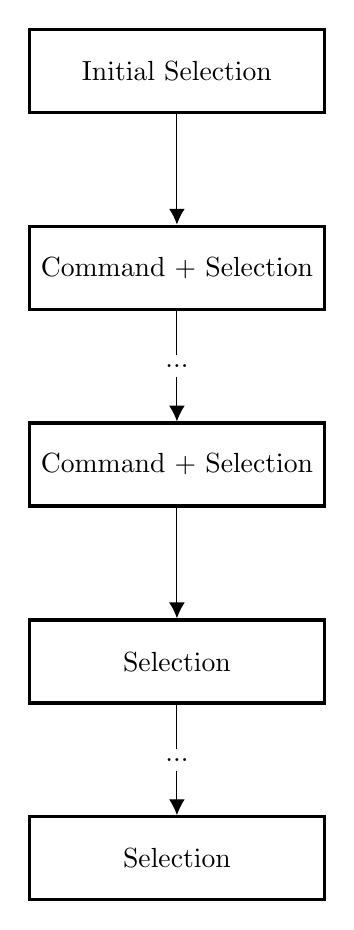
\begin{tikzpicture}
[node distance=2.5cm, every node/.style={fill=white}, align=center]]
\node[box1] (init) {Initial Selection};
\node[box1, below of=init] (a) {Command + Selection};
\node[box1, below of=a] (b) {Command + Selection};
\node[box1, below of=b] (c) {Selection};
\node[box1, below of=c] (d) {Selection};
\draw[->] (init) -- (a);
\draw[->] (a) -- node{...} (b);
\draw[->] (b) -- (c);
\draw[->] (c) -- node{...} (d);
\end{tikzpicture}
\caption{History Structure}
\end{figure}

The structure stores the initial selection and the selection that was used to invoke each command. Each command is expected to update the selection for both \texttt{execute()} and \texttt{undo()} methods, and therefore only one selection needs to be stored per command. Sometimes the selection does not change between commands and only the most recent command needs to store a selection.

Let \texttt{can\_undo} and \texttt{can\_undo} be booleans that determine if the selection needs to be changed before a command can be undone or redone.

\begin{enumerate}
\item \textbf{(add)} If a selection is added, then \texttt{can\_undo = false} and \texttt{can\_redo = false}.
\item \textbf{(add)} If a command is added, then \texttt{can\_undo = true} and \texttt{can\_redo = false}. If no selection has been added since the last command, then remove the selection of the last command.
\item \textbf{(undo)} If \texttt{can\_undo == true}, then \texttt{past.last().command.undo()}. Move the command to the future and set \texttt{can\_undo = !past.last().hasSelection()} and \texttt{can\_redo = true}. If \texttt{can\_undo == true}, then move the current selection to the last memento in \texttt{past}.
\item \textbf{(undo)} If \texttt{can\_undo == false}, then undo the selection. If the new selection has a command, then \texttt{current = true}. Set \texttt{can\_redo = false}.
\item \textbf{(redo)} \ldots
\end{enumerate}

\section{Generator}

\subsection{Stems}

The positions of stems are stored as distances along parent stems. Stems internally calculate vector positions (\textit{i.e.} locations in world space) when distances are changed and when paths of ancestor stems are changed.

\textbf{(TODO)} A map that pairs memory addresses with stem IDs is stored within each plant object so that is possible to quickly reference stems without storing their memory addresses. Entries are added to the map when stems are added to the plant and removed from the map when stems are removed from the plant. This enables objects to manage their own stem copies without leaking memory and preserves selection information after the program exits.

\subsection{Materials/Textures}

The plant object stores a list of all materials that stems and leaves can have. Stems and leaves store IDs of materials (instead of actual material objects), so materials only have to be updated in the plant object. An ID with a value of zero means that the stem or leaf has no material.

The geometry generator needs to create vertex seams (\textit{i.e.} duplicate vertices) so that textures can be wraped around the stems. Vertex seams might not be needed if a special fragment shader is used.

\section{Shaders}

\subsection{Outlines}

Selected objects are indicated with an outline around their silhouette. The outline is achieved in two passes. The first pass draws the selected objects offscreen in solid white onto a black background. This image is stored in a texture for the second pass. During the second pass, the fragment shader refers to this texture to determine if a fragment is close to the object's silhouette edge. Even though the fragment shader needs to scan and analyze the texture, it needs to avoid branch divergence in order to keep performance acceptable.

\end{document}
